%!TEX root = main.tex

\section{Analysis of Web Search Flows}
\label{sec:web_search}

% In this section, 

\subsection{Analysis Framework}

We divide the analysis of web search flow into 3 different pieces corresponding to the three subsequent stages: \emph{3-way handshake}, \emph{slow start}, \emph{congestion avoidance}, in which web server has different transmission strategies.

In TCP 3-way handshake, server establishes connection with client, in preparation for data transmission. Ideally, this stage completes in 1 RTT. However, in the dataset we could see that a non-negligible fraction of flows experience SYN retransmission in 3-way handshake. In slow start stage, server does not encounter packet loss or reordering event. Thus it enlarges the congestion window by 1 segment size for each received acknowledgment, and transmits data constrained by the window size. Server leaves slow start and enters congestion avoidance stage when it encounters congestion event, like packet loss or reordering. In congestion avoidance stage, server reduces the congestion window when detecting packet loss through fast retransmit\cite{jacobson1988congestion} and compels the congestion window to grow from 1 segment size when detecting packet loss through RTO. If there is no congestion event, the flow will complete in slow start stage. It is worth noting that, different from the TCP congestion avoidance state in TCP/IP stack, the \emph{congestion avoidance} stage here starts when server detects congestion event and ends till the flow finishes. 

The three stages could be exemplified in Figure~\ref{fig:web_three_stages}, which shows the time-line and sequence number of a real flow in web search. In the figure, server takes 1.8s to establish connection, 3.1s to transmit 35 data packets in slow start stage, and 15.3s to transmit the left 48 data packets in congestion avoidance stage.

\begin{figure}[th]
\centering
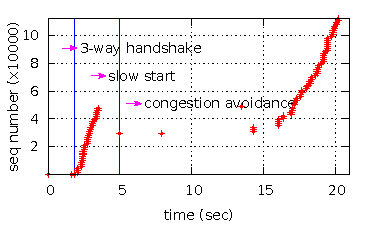
\includegraphics[width=\linewidth]{web_three_stages}
\caption{The three stages in web search flows.}
\label{fig:web_three_stages}
\end{figure}

\subsection{Analyzing the impact on Finish Time}

\begin{figure}[th]
\centering
	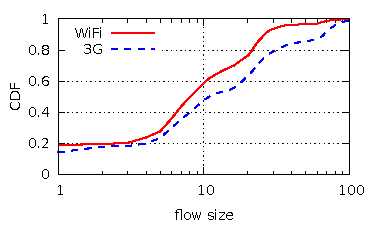
\includegraphics[width=0.8\linewidth]{web_flow_size}
\caption{The distribution of flow sizes in web search.}
\label{fig:web_flow_size}
\end{figure}

In this section, we first study the impact of flow size on finish time in web search flows. Figure~\ref{fig:web_flow_size} shows the distribution of flow sizes in web search.  From the figure, all flows are with less than 100 data packets, in which a large fraction of flows are with size in range between 4 and 30 packets. There are also flows with no search result, resulting in one data packet in the flow, which occupy 15\% of flows. The median value of flow size in WiFi network is smaller than that of flows in 2G/3G network. This may be induced by different customized designs for different access types.

The flow size in web search ranges from 1 to 100 packets. This means that the data could be transmitted in 1 RTT at least, and more than 4 RTT at most. Considering the various flow sizes, the metric $finish\_time$ could not portray the efficiency that the data is delivered. To eliminate the affect of flow size, we introduce one more performance metric transmission time per packet ($tpp$), defined as the average time to transmit a data packet. The metric $tpp$ could be represented as $\frac{finish\_time}{\#(pkts)}$. In the following, we mainly use transmission time per packet ($tpp$) to depict the performance of web search.

\begin{figure}[th]
\centering
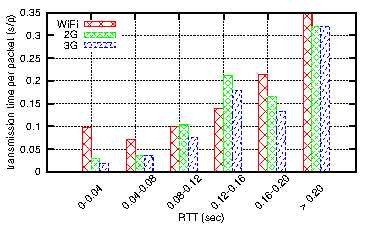
\includegraphics[width=\linewidth]{web_rtt}
\caption{The average transmission time per packet under different RTT's.}
\label{fig:web_rtt}
\end{figure}

First, we investigate the impact of RTT on the transmission time per packet ($tpp$) of web search flows. We also use 0.4s interval to group the flows by their RTT's. The result is shown in Figure~\ref{fig:web_rtt}. From the figure, as the RTT value becomes larger, the overall $tpp$ grows correspondingly. For smaller RTT value (less than 0.08s), the $tpp$ value of flows in WiFi network is 1-4 times larger than that of flows in cellular network. When the RTT value is larger than 0.08s, flows in all networks have similar $tpp$ values. Note that most of flows (95\%) in cellular network have RTT smaller than 0.08s, which verifies that the $tpp$ value of flows in cellular is much lower than that of flows in WiFi network in Figure~\ref{fig:web_finish_time}.

\begin{table}[th]
\centering
\renewcommand{\arraystretch}{1.2}
\caption{Transmission time per packet under different RTT values in cellular network using QED.}
\label{tab:web_cellular_rtt_qed}
\begin{tabular}{l|c|c}
\toprule
RTT bin (s) & 2G & 3G \\
\midrule
$[$ 0.01, 0.02 ) & 11.1 & 6.6 \\
\hline
$[$ 0.02, 0.03 ) & 28.0 & 32.3 \\
\hline
$[$ 0.03, 0.04 ) & 25.1 & 22.4 \\
\hline
$[$ 0.04, 0.05 ) & 67.0 & 59.2 \\
\hline
$[$ 0.05, 0.06 ) & 60.5 & 59.0 \\
\hline
$[$ 0.06, 0.07 ) & 38.6 & 38.8 \\
\hline
$[$ 0.07, 0.08 ) & 69.7 & 39.0 \\
\hline
$[$ 0.08, $\infty$ ) & 581.8 & 317.6 \\
\bottomrule
\end{tabular}
\end{table}

Due to the different distribution of RTT's in cellular network and WiFi network, we investigate the impact of RTT separately. In cellular network data, we use 0.01s interval to group the flows into 9 bins, and take the flows in bin $[$ 0, 0.01 ) as the baseline. For each flow in the baseline, we randomly choose such a flow which has the same access type, the same number of lost packets, and the same condition whether encountering RTO, in each of other bins, and compute the ratio of their $tpp$ values to that of the baseline flow. The results are shown in Table~\ref{tab:web_cellular_rtt_qed}. From the table, the $tpp$ value of flows with RTT larger than 0.01s is much larger than that of flow with RTT smaller than 0.01s. However, we could not find the evidence in the table that $tpp$ value is proportional to RTT value in web search. We also use 0.01s interval to bin the flows in WiFi network into 21 groups. The results are not shown due to space limit. In WiFi network, when the RTT is between 0.04s and 0.16s, the $tpp$ value is not proportional to RTT, either. 

\begin{figure}[th]
\centering
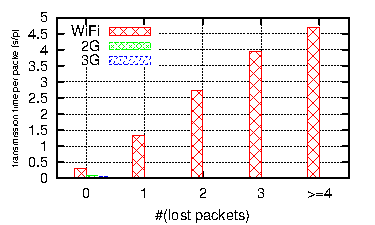
\includegraphics[width=\linewidth]{web_loss_finish_time}
\caption{Transmission time per packet under different number of lost packets.}
\label{fig:web_loss_finish_time}
\end{figure}

Next, we investigate the impact of packet loss on the transmission time per packet ($tpp$). Note that the packet loss rate in 2G/3G network is less than 0.005\%, thus the impact in cellular network could be omitted. In contrast, about 5\% of flows in WiFi network encounter packet loss. Figure~\ref{fig:web_loss_finish_time} plots the $tpp$ values under different number of lost packets. In the figure, when there is no packet loss, the performance of each access type could be ranked as: 3G $>$ 2G $>>$ WiFi. In WiFi network, when the number of lost packets is larger than 3, the $tpp$ value is 15 times larger than that with no packet loss.

\begin{figure}[th]
\centering
	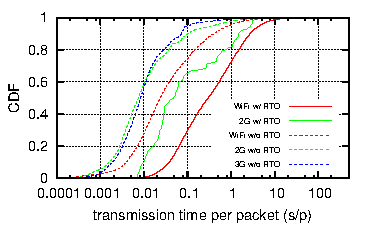
\includegraphics[width=\linewidth]{web_timeout}
\caption{Transmission time per packet of flows with and without timeout retransmission.}
\label{fig:web_timeout}
\end{figure}

Even though flows in 2G network seldom encounters packet loss, 0.7\% of them suffer from timeout retransmission due to packet delay or lost acknowledgment. Figure~\ref{fig:web_timeout} shows the $tpp$ value of flows with and without timeout retransmission. In the figure, under the same access type (WiFi and 2G network), the $tpp$ value of flows with timeout retransmission is one order of magnitude larger than those without timeout retransmission. Considering flows with timeout retransmission, flows in 2G network have smaller $tpp$ value than those in WiFi network. The reasons are as follows. First, flows in 2G network have smaller RTT, and thus smaller RTO according to \cite{rfc62982011computing}. Second, many timeout retransmissions in 2G network are spurious due to packet delay or lost acknowledgment. When receiving Duplicate SACK if the first packet is not dropped, server recovers the original congestion window using F-RTO~\cite{sarolahti2005forward}, instead of increasing the window from 1 segment size.

\begin{figure}[th]
\centering
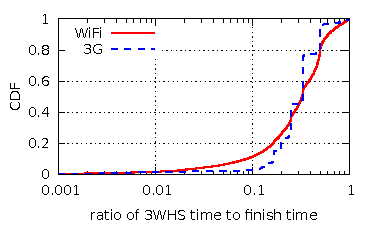
\includegraphics[width=\linewidth]{web_handshake_time_ratio}
\caption{The ratio of time in 3-way handshake to finish time in each flow.}
\label{fig:web_handshake_ratio}
\end{figure}

Next, we break the analysis down into the three stages that flows experience. In Figure~\ref{fig:web_handshake_ratio}, we plot the ratio of time consumed by 3-way handshake to the finish time. From the figure, flows in cellular network have similar ratio of time in 3-way handshake to that in WiFi network (with median value 0.3). If the 3-way handshake could be removed from finish time by some means, the user-perceived performance would be improved by 30\%. Here we also count the percentage of flows with SYN retransmission, which is shown in Table~\ref{tab:web_syn_retrans}. 4.4\% of flows in WiFi network also suffer from timeout retransmission in 3-way handshake stage.

\begin{table}[th]
\centering
\renewcommand{\arraystretch}{1.2}
\caption{Percentage of flows that experience SYN retransmission in web search.}
\label{tab:web_syn_retrans}
\begin{tabular}{l|c|c|c}
\toprule
& WiFi & 2G & 3G \\
\midrule
SYN retransmission & 4.4\% & 2\% & 0.5\% \\
\bottomrule
\end{tabular}
\end{table}

\begin{figure}[th]
\centering
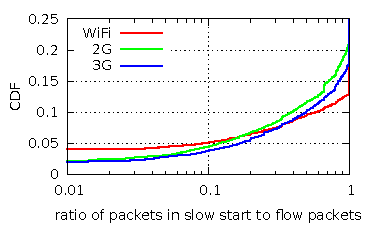
\includegraphics[width=\linewidth]{web_slowstart_pkt_ratio}
\caption{The ratio of packets in slow start to flow packets.}
\label{fig:web_slowstart_ratio}
\end{figure}

Figure~\ref{fig:web_slowstart_ratio} shows the ratio of packets in slow start stage to flow packets. In the figure, a non-negligible fraction of flows (4\% in WiFi, and 2\% in cellular network) do not transmit any packets successfully in slow start stage. Compared to flows in cellular network, flows in WiFi network experience higher packet loss rate, yet 87.5\% of them could transmit all the data packets in slow start stage, larger than those in cellular network (80\% and 83\%). This could be explained as follows. Flow leaves slow start stage when encountering packet reordering or RTO. Cellular network have more packet reordering events than WiFi network.

\begin{table}[th]
\centering
\renewcommand{\arraystretch}{1.2}
\caption{Percentage of flows with packet reordering.}
\label{tab:web_reordering}
\begin{tabular}{l|c|c|c}
\toprule
& WiFi & 2G & 3G \\
\midrule
packet reordering & 9.96\% & 23.0\% & 19.4\% \\
\bottomrule
\end{tabular}
\end{table}

Table~\ref{tab:web_reordering} shows the percentage of web search flows with packet reordering. In the table, more than 20\% of flows in cellular network encounter packet reordering, while the ratio in WiFi network is only 10\%.

\subsection{Summary of Web Search Analysis}

The key observations on web search flows are summarized below.

\begin{itemize}
	\item Compared to the impact of RTT on voice recognition flow, RTT has limited affect on the transmission time per packet in web search.
	\item More than 50\% of flows spend 30\% of their total time on establishing connections.
	\item Flows in WiFi network are more likely to have lost packets, while flows in cellular network have more disordered packets.
	\item Even though 2G network has quite low packet loss rate (0.005\%), 0.7\% of flows encounter timeout retransmission, due to packet reordering.
\end{itemize}